\section{实验}

\subsection{设置与重放合同}

模型为Meta-Llama-3.1-8B-Instruct，source为已审计task group-scale端点。开放layers 28--31的28个Linear、145,465,344个六维向量。ARC-C、ARC-E、HellaSwag、PIQA、WinoGrande各用512/256/31条train/validation/audit；文本为4096/128/64条长度4096的互斥序列。实验固定四视图、8-way邻域和128/Linear bundle，不扫描seed、budget、顺序、阈值、LR或group。只用本机GPU7单卡，耗时3.515小时、峰值25.285GiB。

Parity覆盖32例、长度11--163，cache与同batch完整HF前向最大score误差$1.1444\times10^{-5}$且argmax 32/32一致。旧direct block缺少causal mask的问题已由逐层测试修复；失败run发生在搜索前，不作为方法结果。

\subsection{条件收益与正控制}

\begin{figure}[t]
\centering
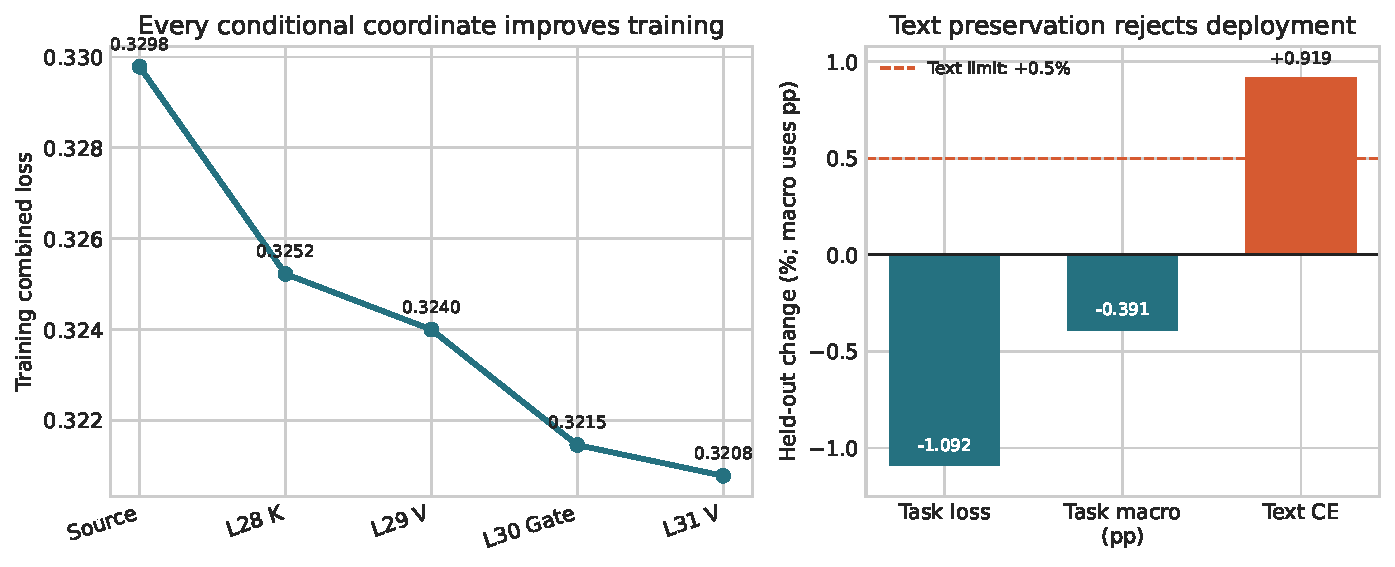
\includegraphics[width=\linewidth]{../img/v13_conditional_gain.pdf}
\caption{四个集合条件坐标均降低训练目标，但文本validation超过预注册退化上限。}
\label{fig:v13}
\end{figure}

\begin{table}[t]
\centering
\small
\caption{每层接受坐标、条件增益与局部正控制。}
\begin{tabular}{llrr}
\toprule
层 & Linear & 条件增益 & Spearman\\
\midrule
28 & K projection & 0.004559 & 0.9643\\
29 & V projection & 0.001224 & 0.3571\\
30 & MLP gate & 0.002538 & 0.5714\\
31 & V projection & 0.000678 & 0.8214\\
\bottomrule
\end{tabular}
\end{table}

四层各接受128个switch，训练联合目标从0.329784依次降至0.325225、0.324001、0.321463、0.320785，总体改善2.7288\%。这证明真实条件评估能在当前四层固定bundle设置中把局部bundle转化为训练收益。每层正控制仅含七个Linear候选，曲率--block MSE相关只能作方向诊断；其跨层波动仍支持局部曲率适合proposal而不能替代端到端裁决。

\subsection{Held-out任务与文本门禁}

\begin{table}[t]
\centering
\small
\caption{Source与条件搜索端点；候选因文本门禁失败而未部署。}
\begin{tabular}{lrrr}
\toprule
指标 & Source & Selected & 变化\\
\midrule
Train joint loss & 0.329784 & \textbf{0.320785} & $-2.7288\%$\\
Val task loss & 0.679691 & \textbf{0.672270} & $-1.0919\%$\\
Val task Macro & \textbf{76.3281} & 75.9375 & $-0.3906$ pp\\
Val text CE & \textbf{2.441416} & 2.463844 & $+0.9186\%$\\
\bottomrule
\end{tabular}
\end{table}

任务门禁通过：held-out balanced loss改善，Macro下降在1 pp容忍内，逐任务loss也没有越线。但文本CE恶化0.9186\%，超过0.5\%上限；训练内部teacher KL也从0.344850上升到0.420074。Task-only标量目标允许supervised收益购买语言分布退化。

\subsection{终态、基线边界与局限}

文本Gate失败后audit未访问、checkpoint未写、WikiText2 PPL和六任务lm\_eval未运行；终态为\texttt{set\_conditional\_gain\_rejected}。V13没有新部署端点，不能声称超过QTIP或GSQ。实验只覆盖一个8B Instruct模型最后四层，任务标签监督也与通用PTQ不同。更早依赖direct DecoderLayer重放的代理证据未采用本版causal-mask parity合同，不能由本次修复追溯性认证；已有完整HF硬验证不受影响。结果只证明当前task-only接受规则不足，不是否定受约束或多目标assignment搜索。
